\section{Theory (50pt)}

To answer questions in this part, you need some basic knowledge of linear algebra and matrix calculus. Also, you need to follow the instructions:
\begin{enumerate}
\item Every vector is treated as column vector.
\item You need to use the numerator-layout notation for matrix calculus. Please refer to  \href{https://en.wikipedia.org/wiki/Matrix_calculus#Numerator-layout_notation}{Wikipedia} about the notation.
\item You are only allowed to use vector and matrix.
You cannot use tensor in any of your answer.
\item Missing transpose are considered as wrong answer.
\end{enumerate}

\subsection{Two-Layer Neural Nets}


You are given the following neural net architecture:
%
\[
\texttt{Linear}_1 \to f \to \texttt{Linear}_2 \to g
\]
%
where $\texttt{Linear}_i (x) = \bm{W}^{(i)}\bm x + \bm b^{(i)}$ is the $i$-th affine transformation, and $f, g$ are element-wise nonlinear activation functions.
When an input $\bm x \in \R^n$ is fed to the network, $ \bm {\hat{y}} \in \R^K$ is obtained as the output.

\subsection{Regression Task}
We would like to perform regression task.
We choose $f(\cdot) = (\cdot)^+ = \texttt{ReLU}(\cdot)$ and $g$ to be the identity function.
To train this network, we choose MSE loss function $\ell_\text{MSE}(\bm{\hat{y}}, \bm{y}) = \| \bm{\hat{y}} - \bm{y} \|^2$, where $y$ is the target output.

\begin{enumerate}[(a)]
\item
(1pt) Name and mathematically describe the 5 programming steps you would take to train this model with \texttt{PyTorch} using SGD on a single batch of data.

\item
(5pt) For a single data point $(x, y)$, write down all inputs and outputs for forward pass of each layer. You can only use variable $ \bm{x}, \bm{y}, \bm{W}^{(1)}, \bm{b}^{(1)}, \bm{W}^{(2)}, \bm{b}^{(2)}$ in your answer. (note that $\texttt{Linear}_i (\bm{x}) = \bm{W}^{(i)}\bm{x} + \bm{b}^{(i)}$).


\begin{center}
\begin{tabular}{ |c |c |c | }
\hline
Layer & Input & Output \\
\hline
$\texttt{Linear}_1$ &  &  \\
\hline
$f$ &  &  \\  
\hline
$\texttt{Linear}_2$ & &  \\
\hline
$g$ &  &  \\
\hline
\texttt{Loss} &  &  \\
\hline
\end{tabular}
\end{center}


\item
(8pt) Write down the gradient calculated from the backward pass. You can only use the following variables: $\bm{x}, \bm{y}, \bm{W}^{(1)}, \bm{b}^{(1)}, \bm{W}^{(2)}, \bm{b}^{(2)}, \frac{\partial \ell}{\partial \bm{\hat y}}, \frac{\partial \bm{z}_2}{\partial \bm{z}_1}, \frac{\partial \bm{\hat y}}{\partial \bm{z_3}}$ in your answer, where $\bm{z}_1, \bm{z}_2, \bm{z}_3, \bm{\hat y}$ are the outputs of $\texttt{Linear}_1, f, \texttt{Linear}_2, g$.

\begin{center}
\begin{tabular}{ |c |c | }
\hline
Parameter &  Gradient \\
\hline
$W^{(1)}$ &\\
\hline
$b^{(1)}$ &  \\ 
\hline
$W^{(2)}$ &  \\
\hline
$b^{(2)}$ & \\
\hline
\end{tabular}
\end{center}

\item 
(3pt) Show us the elements of $\frac{\partial \bm{z_2}}{\partial \bm{z_1}}$, $\frac{\partial \bm{\hat y}}{\partial \bm{z_3}}$ and $\frac{\partial \ell}{\partial \bm{\hat y}}$ (be careful about the dimensionality)?

\end{enumerate}


\textbf{Solution:}

(a)
\begin{enumerate}
% \item 
\item Generate a prediction ($\hat{y} = model(x)$)
\item Compute the loss function (loss = criterion($\hat{y}$, $y$))
\item zero $\nabla params$, clear the gradients of all parameters. (optimizer.zero\_grad())
\item Compute and Accumulate $\nabla params$: Backpropagation to compute the gradients of the loss function with respect to the parameters. (loss.backward())
\item Step in towards -$\nabla params$: Update the parameters and update the optimizer status. (optimizer.step())
\end{enumerate}


(b)

$ \bm{x}, \bm{y}, \bm{W}^{(1)}, \bm{b}^{(1)}, \bm{W}^{(2)}, \bm{b}^{(2)}$

For a single data point $(x, y)$, we have:

\begin{center}
    \begin{tabular}{ |c |c |c | }
    \hline
    Layer & Input & Output \\
    \hline
    $\texttt{Linear}_1$ & $\bm{x}$ & $\bm{W}^{(1)}\bm{x} + \bm{b}^{(1)}$ \\
    \hline
    $f$ & $\bm{W}^{(1)}\bm{x} + \bm{b}^{(1)}$ & $f(\bm{W}^{(1)}\bm{x} + \bm{b}^{(1)})$ \\  
    \hline
    $\texttt{Linear}_2$ & $f(\bm{W}^{(1)}\bm{x} + \bm{b}^{(1)})$ & $\bm{W}^{(2)}f(\bm{W}^{(1)}\bm{x} + \bm{b}^{(1)}) + \bm{b}^{(2)}$ \\
    \hline
    $g$ & $\bm{W}^{(2)}f(\bm{W}^{(1)}\bm{x} + \bm{b}^{(1)}) + \bm{b}^{(2)}$ & $\bm{W}^{(2)}f(\bm{W}^{(1)}\bm{x} + \bm{b}^{(1)}) + \bm{b}^{(2)}$ \\
    \hline
    \texttt{Loss} & $\bm{W}^{(2)}f(\bm{W}^{(1)}\bm{x} + \bm{b}^{(1)}) + \bm{b}^{(2)}$  & $\| \bm{W}^{(2)}f(\bm{W}^{(1)}\bm{x} + \bm{b}^{(1)}) + \bm{b}^{(2)}  - \bm{y} \|^2$ \\
    \hline
    \end{tabular}
\end{center}

\newpage
The input dim is n, the output dim is k, we define the output dim of middle layer as L1, L2=K. We have B = batch-size = 1 here, so we have:

x.shape = (feature-in, batch-size) = (n, B) 

W1.shape = (L1, n)

b1.shape = (L1)

z1.shape = (W1 x + b1).shape = (L1, B)

z2.shape = f(z1).shape = (L1, B)

W2.shape = (K, L1)

b2.shape = (K)

z3.shape = (W2 x + b2).shape = (K, B)

y\_hat.shape = g(z3).shape = (K, B)


(c)


\begin{center}
    \begin{tabular}{ |c |c | }
    \hline
    Parameter &  Gradient \\
    \hline
    $W^{(1)}$ & $  \frac{\partial \bm{z_2}}{\partial \bm{z_1}}  (\bm{(W^{(2)})}^T ( \frac{\partial \bm{\hat y}}{\partial \bm{z_3}} \frac{\partial \ell}{\partial \bm{\hat y}})) \bm{x}^T $\\
    \hline
    $b^{(1)}$ & $  \frac{\partial \bm{z_2}}{\partial \bm{z_1}} (\bm{(W^{(2)})}^T (\frac{\partial \bm{\hat y}}{\partial \bm{z_3}} \frac{\partial \ell}{\partial \bm{\hat y}} ))  \frac{\partial \bm{z_2}}{\partial \bm{z_1}} $ \\ 
    \hline
    $W^{(2)}$ & $ \frac{\partial \bm{\hat y}}{\partial \bm{z_3}} \frac{\partial \ell}{\partial \bm{\hat y}} (f(\bm{W}^{(1)}\bm{x} + \bm{b}^{(1)}))^T$  \\
    \hline
    $b^{(2)}$ & $  \frac{\partial \bm{\hat y}}{\partial \bm{z_3}}\frac{\partial \ell}{\partial \bm{\hat y}}$\\
    \hline
    \end{tabular}
\end{center}

\textbf{We use matrix multiplication in the activation gradient backpropagation, the gradient of activation funcation is a diagonal matrix.}

For $\frac{\partial \bm{\hat y}}{\partial \bm{z_3}}\frac{\partial \ell}{\partial \bm{\hat y}}$, which is equvalent to $\frac{\partial \ell}{\partial \bm{\hat y}} \cdot f'(z_3)$ , which is
\begin{align}
    &\frac{\partial \ell}{\partial \bm{\hat y}} \cdot g'(z_3)
= \frac{\partial \ell}{\partial \bm{\hat y}} \cdot     
\left[
    \begin{array}{c}
        1 \\
        1 \\
        \vdots \\
        1
    \end{array}
\right] \\
&\equiv \frac{\partial \bm{\hat y}}{\partial \bm{z_3}}\frac{\partial \ell}{\partial \bm{\hat y}} = I_{K} \frac{\partial \ell}{\partial \bm{\hat y}}\\
&\equiv  \frac{\partial \bm{\hat y}}{\partial \bm{z_3}}  \frac{\partial \ell}{\partial \bm{\hat y}}
= \left[
    \begin{array}{cccc}
        1 & 0 & \vdots & 0 \\
        0 & 1 & \vdots & 0 \\
        \vdots & \vdots & \vdots & \vdots \\
        0 & 0 & \vdots & 1 
    \end{array}
\right] \frac{\partial \ell}{\partial \bm{\hat y}}
\end{align}



\begin{equation}
    \bm{y} = [y_1, y_2, ..., y_n]^T
\end{equation}

\begin{equation}
    \frac{\partial \ell}{\partial \bm{\hat y}} = 2( \bm{\hat{y}} - \bm{y})
\end{equation}

$y \in \R^{K \times 1}$

\begin{equation}
    \frac{\partial \ell}{\partial \bm{z_3}} = \frac{\partial \ell}{\partial \bm{\hat y}} \frac{\partial \bm{\hat y}}{\partial \bm{z_3}} = 2( \bm{\hat{y}} - \bm{y})
\end{equation}


\begin{align}
    \frac{\partial \ell}{\partial \bm{W^{(2)}}} 
    &= \frac{\partial \ell}{\partial \bm{\hat y}} \frac{\partial \bm{\hat y}}{\partial \bm{z_3}} \frac{\partial \bm{z_3}}{\partial \bm{W^{(2)}}}  \\
    &= \frac{\partial \ell}{\partial \bm{\hat y}} \frac{\partial \bm{\hat y}}{\partial \bm{z_3}} \bm{z_2}^T \\
    &= \frac{\partial \bm{\hat y}}{\partial \bm{z_3}} \frac{\partial \ell}{\partial \bm{\hat y}}  (f(\bm{W}^{(1)}\bm{x} + \bm{b}^{(1)}))^T \\
\end{align}

% $[L2 * 1] @ [L1 * 1]^T = [L2 * L1]$


\begin{align}
    \frac{\partial \ell}{\partial \bm{b^{(2)}}} 
    &= \frac{\partial \ell}{\partial \bm{\hat y}} \frac{\partial \bm{\hat y}}{\partial \bm{z_3}} \frac{\partial \bm{z_3}}{\partial \bm{b^{(2)}}}  \\
    &= \frac{\partial \bm{\hat y}}{\partial \bm{z_3}}   \frac{\partial \ell}{\partial \bm{\hat y}} 
\end{align}

\begin{align}
    \frac{\partial \ell}{\partial \bm{W^{(1)}}} 
    &= \frac{\partial \ell}{\partial \bm{\hat y}} \frac{\partial \bm{\hat y}}{\partial \bm{z_3}} \frac{\partial \bm{z_3}}{\partial \bm{z_2}} \frac{\partial \bm{z_2}}{\partial \bm{z_1}} \frac{\partial \bm{z_1}}{\partial \bm{W^{(1)}}}  \\
    &= \frac{\partial \bm{z_2}}{\partial \bm{z_1}}  (\bm{(W^{(2)})}^T ( \frac{\partial \bm{\hat y}}{\partial \bm{z_3}} \frac{\partial \ell}{\partial \bm{\hat y}})) \bm{x}^T\\ 
    % &= 2( \bm{\hat{y}} - \bm{y})^T \bm{W^{(2)}}  \frac{\partial \bm{z_2}}{\partial \bm{z_1}} \bm{x}^T \\
\end{align}

% $[L2] @ [L2, L1] @ [L1, L1] @ [n] = [, n]$

$\bm{\hat y} \in \R^{K \times 1}$, $\bm{z_3} \in \R^{K \times 1}$, $\frac{\partial \bm{\hat y}}{\partial \bm{z_3}} \in \R^{K \times K}$.

\begin{equation}
    \frac{\partial \ell}{\partial \bm{b^{(1)}}} = (\frac{\partial \bm{\hat y}}{\partial \bm{z_3}} \frac{\partial \ell}{\partial \bm{\hat y}} ) \frac{\partial \bm{z_3}}{\partial \bm{z_2}} \frac{\partial \bm{z_2}}{\partial \bm{z_1}} \frac{\partial \bm{z_1}}{\partial \bm{b^{(1)}}} = \frac{\partial \bm{z_2}}{\partial \bm{z_1}}  (\bm{(W^{(2)})}^T ( \frac{\partial \bm{\hat y}}{\partial \bm{z_3}} \frac{\partial \ell}{\partial \bm{\hat y}})) 
\end{equation}


(d)

% Show us the elements of $\frac{\partial \bm{z_2}}{\partial \bm{z_1}}$, $\frac{\partial \bm{\hat y}}{\partial \bm{z_3}}$ and $\frac{\partial \ell}{\partial \bm{\hat y}}$ (be careful about the dimensionality)?



If we only consider one data point,

% z2.shape = (linear2-out, 1)

% z1.shape = (linear1-out, 1)

z1 = w1 * x + b1

z2 = f(z1)

z3 = W2 * z2 + b2

y\_hat = g(z3)

% \linebreak 

$\bm{z_2} \in \R^{L_1} $, $\bm{z_1} \in \R^{L_1} $, $\frac{\partial \bm{z_2}}{\partial \bm{z_1}} \in \R^{L1 \times L1}$, vector by vector derivative.

\begin{equation}
    \frac{\partial \mathbf{z_2}}{\partial \mathbf{z_1}}
    =
    % \frac{\partial \mathbf{y}}{\partial \mathbf{x}}=
    \left[\begin{array}{cccc}
        \frac{\partial z_{2}{[1]}}{\partial z_{1}{[1]}} & \frac{\partial z_{2}{[2]}}{\partial z_{1}{[1]}} & \cdots & \frac{\partial z_{2}{[L1]}}{\partial z_{1}{[1]}} \\
        \frac{\partial z_{2}{[1]}}{\partial z_{1}{[2]}} & \frac{\partial z_{2}{[2]}}{\partial z_{1}{[2]}} & \cdots & \frac{\partial z_{2}{[L1]}}{\partial z_{1}{[2]}} \\
        \vdots & \vdots & \ddots & \vdots \\
        \frac{\partial z_{2}{[1]}}{\partial z_{1}{[L1]}} & \frac{\partial z_{2}{[2]}}{\partial z_{1}{[L1]}} & \cdots & \frac{\partial z_{2}{[L1]}}{\partial z_{1}{[L1]}}
    \end{array}\right]
    = 
    \left[
        \begin{array}{cccc}
            \mathbb{1} z_{2_{1} > 0} & 0 & \cdots & 0 \\
            0 & \mathbb{1} z_{2_{2} > 0} & \cdots & 0 \\
            \vdots & \vdots & \ddots & \vdots \\
            0 & 0 & 0 &\mathbb{1} z_{2_{L1} > 0}  
        \end{array}
    \right]
\end{equation}

For the element in the matrix, if the corrosponding element in the $\bm{z_2}$ is greater than 0, then the element in the matrix is 1, otherwise it is 0.


% $\mathbf{z_2} \in \R^{L2} $, $\mathbf{z_1} \in \R^{L1}$, $\frac{\partial \mathbf{z_2}}{\partial \mathbf{z_1}} \in \R^{L2 \times L1} $ 

$\frac{\partial \bm{\hat y}}{\partial \bm{z_3}}$,  vector-by-vector derivative

% \text{NOT Sure why use $\textbf{y}$ in the questions satement, we take $\textbf{y}$ as vector here,}

\begin{equation}
    \frac{\partial \mathbf{\hat{y}}}{\partial \mathbf{z_3}}
    % =\left[\begin{array}{cccc}
    % \frac{\partial \hat{y}_{1}}{\partial z_{{3}_{1}}} & \frac{\partial \hat{y}_{1}}{\partial z_{{3}_{2}}} & \cdots & \frac{\partial \hat{y}_{1}}{\partial z_{{3}_{K}}} \\
    % \frac{\partial \hat{y}_{2}}{\partial z_{{3}_{1}}} & \frac{\partial \hat{y}_{2}}{\partial z_{{3}_{2}}} & \cdots & \frac{\partial \hat{y}_{2}}{\partial z_{{3}_{K}}} \\
    % \vdots & \vdots & \ddots & \vdots \\
    % \frac{\partial \hat{y}_{K}}{\partial z_{{3}_{1}}} & \frac{\partial \hat{y}_{K}}{\partial z_{{3}_{2}}} & \cdots & \frac{\partial \hat{y}_{K}}{\partial z_{{3}_{K}}}
    % \end{array}\right]
    =
    I_{K}
\end{equation}

$\mathbf{z_3} \in \R^{K} $, $\mathbf{\hat{y}} \in \R^{K}$, $\frac{\partial \mathbf{\hat{y}}}{\partial \mathbf{z_3}} \in \R^{K \times K} $. Only the diagonal elements are one.

% If we only consider one data point and the regression task, the $\frac{\partial \hat{y}}{\partial \mathbf{z_3}}$. 

% \begin{equation}
%     \frac{\partial \hat{y}}{\partial \mathbf{z_3}}=\left[\begin{array}{cccc}
%     \frac{\partial \hat{y}}{\partial z_{{3}_{1}}} & \frac{\partial \hat{y}}{\partial z_{{3}_{2}}} & \cdots & \frac{\partial \hat{y}}{\partial z_{{3}_{K}}} \\
%     \end{array}\right]
% \end{equation}


$\frac{\partial \ell}{\partial \bm{\hat y}}$, scalar-by-vector derivative.

\begin{equation}
    \frac{\partial \ell }{\partial \mathbf{\hat{y}}}=\left[\begin{array}{cccc}
    \frac{\partial \ell}{\partial \hat{y}_{1}} & \frac{\partial \ell}{\partial \hat{y}_{2}} & \cdots & \frac{\partial \ell}{\partial \hat{y}_{K}} \\
    \end{array}\right]^T \\
    = 2 (\mathbf{\hat{y}} - \mathbf{y})
    = 2 \left[\hat{y}_0- {y}_0, \hat{y}_1 - {y}_1  ... \right]^T
\end{equation}

where $\mathbf{y} = [y_0, y_1, ..., y_K]^T$.

$\ell \in \R$, $\mathbf{\hat{y}} \in \R^{K}$, $\frac{\partial \ell}{\partial \mathbf{\hat{y}}} \in \R^{K} $. 
% $\mathbf{z_3} \in \R^{K} $, $\mathbf{\hat{y}} \in \R^{K}$, $\frac{\partial \mathbf{\hat{y}}}{\partial \mathbf{z_3}} \in \R^{K \times K} $.


\subsection{Classification Task}
We would like to perform multi-class classification task, so we set both $f, g = \sigma$, the logistic sigmoid function $\sigma(z) \doteq (1 + \exp(-z))^{-1}$.

\begin{enumerate}[(a)] 
\item
(2pt + 6pt + 2pt) If you want to train this network, what do you need to change in the equations of (b), (c) and (d), assuming we are using the same MSE loss function.

\item
(2pt + 6pt + 2pt) Now you think you can do a better job by using a \emph{Binary Cross Entropy} (BCE) loss function $\ell_\text{BCE}(\bm{\hat{y}}, \bm{y}) = \frac{1}{K}\sum_{i=1}^K -\big[\hat{y}_i \log(\hat{y}_i) + (1 - \hat{y}_i)\log(1 - \hat{y}_i)\big]$.
What do you need to change in the equations of (b), (c) and (d)?

\item
(1pt) Things are getting better.
You realize that not all intermediate hidden activations need to be binary (or soft version of binary).
You decide to use $f(\cdot) = (\cdot)^+$ but keep $g$ as $\sigma$. Explain why this choice of $f$ can be beneficial for training a (deeper) network.


\end{enumerate}

\textbf{Solution:}
\subsubsection{(a)}

\begin{center}
    \begin{tabular}{ |c |c |c | }
    \hline
    Layer & Input & Output \\
    \hline
    $\texttt{Linear}_1$ & $\bm{x}$ & $\bm{W}^{(1)}\bm{x} + \bm{b}^{(1)}$ \\
    \hline
    $f$ & $\bm{W}^{(1)}\bm{x} + \bm{b}^{(1)}$ & $\sigma(\bm{W}^{(1)}\bm{x} + \bm{b}^{(1)})$ \\  
    \hline
    $\texttt{Linear}_2$ & $\sigma(\bm{W}^{(1)}\bm{x} + \bm{b}^{(1)})$ & $\bm{W}^{(2)}\sigma(\bm{W}^{(1)}\bm{x} + \bm{b}^{(1)}) + \bm{b}^{(2)}$ \\
    \hline
    $g$ & $\bm{W}^{(2)}\sigma(\bm{W}^{(1)}\bm{x} + \bm{b}^{(1)}) + \bm{b}^{(2)}$ & $\sigma(\bm{W}^{(2)}\sigma(\bm{W}^{(1)}\bm{x} + \bm{b}^{(1)}) + \bm{b}^{(2)})$ \\
    \hline
    \texttt{Loss} & $\sigma(\bm{W}^{(2)}\sigma(\bm{W}^{(1)}\bm{x} + \bm{b}^{(1)}) + \bm{b}^{(2)})$  & $\| \sigma(\bm{W}^{(2)}\sigma(\bm{W}^{(1)}\bm{x} + \bm{b}^{(1)}) + \bm{b}^{(2)})  - \bm{y} \|^2$ \\
    \hline
    \end{tabular}
\end{center}



% $\bm{x}, \bm{y}, \bm{W}^{(1)}, \bm{b}^{(1)}, \bm{W}^{(2)}, \bm{b}^{(2)}, \frac{\partial \ell}{\partial \bm{\hat y}}, \frac{\partial \bm{z}_2}{\partial \bm{z}_1}, \frac{\partial \bm{\hat y}}{\partial \bm{z_3}}$

Here we do not expand the $\sigma$ to prevent the fomula from becoming too long. Forward table do not change much, only change the f and g to $\sigma$


MSE Loss and f, g = $\sigma$. the gradient table do not changed, but the term $\frac{\partial \bm{z}_2}{\partial \bm{z}_1}$, $\frac{\partial \bm{\hat y}}{\partial \bm{z_3}}$ are changed.

\begin{center}
    \begin{tabular}{ |c |c | }
    \hline
    Parameter &  Gradient \\
    \hline
    $W^{(1)}$ & $  \frac{\partial \bm{z_2}}{\partial \bm{z_1}}  (\bm{(W^{(2)})}^T ( \frac{\partial \bm{\hat y}}{\partial \bm{z_3}} \frac{\partial \ell}{\partial \bm{\hat y}})) \bm{x}^T $\\
    \hline
    $b^{(1)}$ & $  \frac{\partial \bm{z_2}}{\partial \bm{z_1}} (\bm{(W^{(2)})}^T (\frac{\partial \bm{\hat y}}{\partial \bm{z_3}} \frac{\partial \ell}{\partial \bm{\hat y}} ))  \frac{\partial \bm{z_2}}{\partial \bm{z_1}} $ \\ 
    \hline
    $W^{(2)}$ & $ \frac{\partial \bm{\hat y}}{\partial \bm{z_3}} \frac{\partial \ell}{\partial \bm{\hat y}} (f(\bm{W}^{(1)}\bm{x} + \bm{b}^{(1)}))^T$  \\
    \hline
    $b^{(2)}$ & $  \frac{\partial \bm{\hat y}}{\partial \bm{z_3}}\frac{\partial \ell}{\partial \bm{\hat y}}$\\
    \hline
    \end{tabular}
\end{center}

% For the devariation, $\frac{\partial \bm{\hat y}}{\partial \bm{z_3}}$ and $\frac{\partial \bm{z_2}}{\partial \bm{z_1}}$ changed.


For the (d) part, 

$\frac{\partial \bm{z_2}}{\partial \bm{z_1}}$ becomes element-wise $\sigma({z_1}) (1 - \sigma({z_1})) = z_2 (1 - z_2)$


\begin{equation}
    \frac{\partial \mathbf{z_2}}{\partial \mathbf{z_1}}
    =
    % \frac{\partial \mathbf{y}}{\partial \mathbf{x}}=
    \left[\begin{array}{cccc}
        \frac{\partial z_{2}{[1]}}{\partial z_{1}{[1]}} & \frac{\partial z_{2}{[2]}}{\partial z_{1}{[1]}} & \cdots & \frac{\partial z_{2}{[L1]}}{\partial z_{1}{[1]}} \\
        \frac{\partial z_{2}{[1]}}{\partial z_{1}{[2]}} & \frac{\partial z_{2}{[2]}}{\partial z_{1}{[2]}} & \cdots & \frac{\partial z_{2}{[L1]}}{\partial z_{1}{[2]}} \\
        \vdots & \vdots & \ddots & \vdots \\
        \frac{\partial z_{2}{[1]}}{\partial z_{1}{[L1]}} & \frac{\partial z_{2}{[2]}}{\partial z_{1}{[L1]}} & \cdots & \frac{\partial z_{2}{[L1]}}{\partial z_{1}{[L1]}}
    \end{array}\right]
    = 
    \left[
        \small
        \begin{array}{cccc}
            (\bm{z_{2_{[1]}}}) (1 - (\bm{z_{2_{[1]}}}))& 0 & \cdots & 0 \\
            0 & (\bm{z_{2_{[2]}}}) (1 - (\bm{z_{2_{[2]}}})) & \cdots & 0 \\
            \vdots & \vdots & \ddots & \vdots \\
            0 & 0 & \cdots & (\bm{z_{2_{[L1]}}}) (1 - (\bm{z_{2_{[L1]}}})
        \end{array}
    \right]
\end{equation}

    $\frac{\partial \bm{\hat y}}{\partial \bm{z_3}}$ = is changed to element-wise $\sigma({z_3}) (1 - \sigma({z_3})) = {\hat{y}}(1- {\hat y}) $.


    \begin{equation}
        \frac{\partial \mathbf{\hat{y}}}{\partial \mathbf{\hat{z_3}}}
        =
        \left[
            \begin{array}{cccc}
                { \hat{y_1}(1 - {\hat{y_1}}) } & 0 & \cdots & 0 \\
                0 & { \hat{y_2}(1 - {\hat{y_2}}) } & \cdots & 0 \\
                \vdots & \vdots & \ddots & \vdots \\
                0 & 0 & \cdots & { \hat{y_K}(1 - {\hat{y_K}}) }
            \end{array}
        \right]
    \end{equation}


    $\frac{\partial \ell}{\partial \bm{\hat y}} = 2( \bm{\hat{y}} - \bm{y})$ do not change.


\newpage

\subsubsection{(b)}

BCE Loss and f, g = $\sigma$. the gradient table representations do not changed, but the terms $\frac{\partial \ell}{\partial \bm{\hat y}}$, $\frac{\partial \bm{z}_2}{\partial \bm{z}_1}$, $\frac{\partial \bm{\hat y}}{\partial \bm{z_3}}$ are changed.

\begin{center}
    \begin{tabular}{ |c |c |c | }
    \hline
    Layer & Input & Output \\
    \hline
    $\texttt{Linear}_1$ & $\bm{x}$ & $\bm{W}^{(1)}\bm{x} + \bm{b}^{(1)}$ \\
    \hline
    $f$ & $\bm{W}^{(1)}\bm{x} + \bm{b}^{(1)}$ & $\sigma(\bm{W}^{(1)}\bm{x} + \bm{b}^{(1)})$ \\  
    \hline
    $\texttt{Linear}_2$ & $\sigma(\bm{W}^{(1)}\bm{x} + \bm{b}^{(1)})$ & $\bm{W}^{(2)}\sigma(\bm{W}^{(1)}\bm{x} + \bm{b}^{(1)}) + \bm{b}^{(2)}$ \\
    \hline
    $g$ & $\bm{W}^{(2)}\sigma(\bm{W}^{(1)}\bm{x} + \bm{b}^{(1)}) + \bm{b}^{(2)}$ & $\sigma(\bm{W}^{(2)}\sigma(\bm{W}^{(1)}\bm{x} + \bm{b}^{(1)}) + \bm{b}^{(2)})$ \\
    \hline
    \texttt{Loss} & $\sigma(\bm{W}^{(2)}\sigma(\bm{W}^{(1)}\bm{x} + \bm{b}^{(1)}) + \bm{b}^{(2)})$ 
    & $ \frac{1}{K} \sum_{i=1}^{K}-[y_{i} \log (\hat{y}_{i})+(1 - {y}_i)\log(1 - \hat{y}_i) ]$ \\
    \hline
    \end{tabular}
\end{center}

\begin{center}
    \begin{tabular}{ |c |c | }
    \hline
    Parameter &  Gradient \\
    \hline
    $W^{(1)}$ & $  \frac{\partial \bm{z_2}}{\partial \bm{z_1}}  (\bm{(W^{(2)})}^T ( \frac{\partial \bm{\hat y}}{\partial \bm{z_3}} \frac{\partial \ell}{\partial \bm{\hat y}})) \bm{x}^T $\\
    \hline
    $b^{(1)}$ & $  \frac{\partial \bm{z_2}}{\partial \bm{z_1}} (\bm{(W^{(2)})}^T (\frac{\partial \bm{\hat y}}{\partial \bm{z_3}} \frac{\partial \ell}{\partial \bm{\hat y}} ))  \frac{\partial \bm{z_2}}{\partial \bm{z_1}} $ \\ 
    \hline
    $W^{(2)}$ & $ \frac{\partial \bm{\hat y}}{\partial \bm{z_3}} \frac{\partial \ell}{\partial \bm{\hat y}} (f(\bm{W}^{(1)}\bm{x} + \bm{b}^{(1)}))^T$  \\
    \hline
    $b^{(2)}$ & $  \frac{\partial \bm{\hat y}}{\partial \bm{z_3}}\frac{\partial \ell}{\partial \bm{\hat y}}$\\
    \hline
    \end{tabular}
\end{center}

where $$\bm{\hat{y}} = \sigma(\bm{W}^{(2)}\sigma(\bm{W}^{(1)}\bm{x} + \bm{b}^{(1)}) + \bm{b}^{(2)}), \quad \bm{y} \in \R^{K}$$.

$\frac{\partial \bm{\hat{y}}}{\partial \bm{z_3}}$ is changed to the diagonal $\sigma({z_3}) (1 - \sigma({z_3}))$ .


\begin{equation}
    \frac{\partial \mathbf{\hat{y}}}{\partial \mathbf{\hat{z_3}}}
    =
    \left[
        \begin{array}{cccc}
            { \hat{y_1}(1 - {\hat{y_1}}) } & 0 & \cdots & 0 \\
            0 & { \hat{y_2}(1 - {\hat{y_2}}) } & \cdots & 0 \\
            \vdots & \vdots & \ddots & \vdots \\
            0 & 0 & \cdots & { \hat{y_K}(1 - {\hat{y_K}}) }
        \end{array}
    \right]
\end{equation}


$\frac{\partial \bm{z_2}}{\partial \bm{z_1}}$ is changed to the diagonal $\sigma({z_1}) (1 - \sigma({z_1}))$.

\begin{equation}
    \frac{\partial \mathbf{z_2}}{\partial \mathbf{z_1}}
    = 
    \left[
        \small
        \begin{array}{cccc}
            (\bm{z_{2_{[1]}}}) (1 - (\bm{z_{2_{[1]}}}))& 0 & \cdots & 0 \\
            0 & (\bm{z_{2_{[2]}}}) (1 - (\bm{z_{2_{[2]}}})) & \cdots & 0 \\
            \vdots & \vdots & \ddots & \vdots \\
            0 & 0 & \cdots & (\bm{z_{2_{[L1]}}}) (1 - (\bm{z_{2_{[L1]}}})
        \end{array}
    \right]
\end{equation}


\begin{equation}
    \frac{\partial \ell}{\partial \bm{\hat y}}
     = \frac{1}{K} [\frac{{\hat{y_1} - {y_1}}}{ {\hat{y_1}} * (1 - {\hat{y_1}})}, \frac{{\hat{y_2} - {y_2}}}{ {\hat{y_2}} * (1 - {\hat{y_2}})}, ... , \frac{{\hat{y_K} - {y_K}}}{ {\hat{y_K}} * (1 - {\hat{y_K}})}]^T
\end{equation}

$\frac{\partial \ell}{\partial \bm{\hat y}} \in \R^{K}$.


\begin{align}
    \frac{\partial \ell}{\partial \bm{z_3}} 
    &= \frac{\partial \ell}{\partial \bm{\hat y}} \frac{\partial \bm{\hat y}}{\partial \bm{z_3}}          \\
    % &= \frac{\partial \ell}{\partial \bm{\hat y}} 
    %     \hat{y} (1-\hat{y})                      \\
    &=\frac{1}{K}\left[
        \begin{array}{c}
            \hat{y_1} - y_1 \\
            \hat{y_2} - y_2 \\
            \vdots   \\
            \hat{y_K} - y_K
        \end{array}
    \right]
\end{align}

$\frac{\partial \bm{z_2}}{\partial \bm{z_1}}$, 


\begin{equation}
    \frac{\partial \mathbf{{z_2}}}{\partial \mathbf{{z_1}}}
    =
    \left[
        \begin{array}{cccc}
            z_{2_{1}}(1 - z_{2_{1}}) & 0 & \cdots & 0 \\
            0 & z_{2_{2}}(1 - z_{2_{2}}) & \cdots & 0 \\
            \vdots & \vdots & \ddots & \vdots \\
            0 & 0 & \cdots & z_{2_{K}}(1 - z_{2_{K}})
        \end{array}
    \right]
\end{equation}



\subsubsection{(c)}

The advantage of using the ReLU over Sigmoid in the middle layers:
\begin{itemize}
    \item Preventing Small Derivatives: When the value is too large or too small, the derivatives of sigmoid is close to 0, but relu is a non-saturated activation function. This phenomenon does not exist.
    \item Increasing the sparicity of the network: when the value is less than 0, the derivative of relu is 0, and the derivative of sigmoid is close to 0.
\end{itemize}

% This do not limit intermediate features or representations and reserve more information, which make the representations more powerful.

\subsection{Conceptual Questions}

\begin{enumerate}[(a)]
    \item (1pt) Why is softmax actually soft(\textit{arg})max?
    \item (1pt) In what situations, soft(\textit{arg})max can become unstable?
    \item (1pt) Should we have two consecutive linear layers in a neural network? Why or why not? 
    
    \item (4pt) Can you draw the graph of the derivative for the following functions?
    \begin{itemize}
        \item \texttt{ReLU()}
        \item \texttt{LeakyReLU(negative\_slope=0.01)}
        \item \texttt{Softplus(beta=1)}
        \item \texttt{GELU()}
    \end{itemize}
    
    \item (4pt) What are 4 different types of linear transformations? What is the role of linear transformation and non linear transformation in a neural network?
    \item (1pt) How should we adjust the learning rate as we increase or decrease the batch size?
    
    
\end{enumerate}


\textbf{Solution:}

(a)

Soft-\{Function-Name\} is the name of the softened version of the function.

The argmax function takes a vector as input and returns a one-hot vector of the maximum value.

The softmax (softargmax) function is a softened version of this function, which return a distribution but not the value of the maximum value.


(b)

If the maximum value and the minimum value are in quite different scales, the softmax function will become unstable (numerically unstable for values with a very large range). 

(c)

We should not have two consecutive linear layers in a neural network. Two consecutive linear layers can be transfered/merged to a single linear layer.


(d)


ReLU 

\includegraphics[width=\linewidth]{./imgs/relu.png}

LeakyReLU

\includegraphics[width=\linewidth]{./imgs/leakyrelu.png}


\includegraphics[width=\linewidth]{./imgs/leakyrelu_zoomin.png}

Softplus(beta=1)

\includegraphics[width=\linewidth]{./imgs/softplus.png}


% \includegraphics[width=\linewidth]{./imgs/leakyrelu_zoomin.png}



GELU

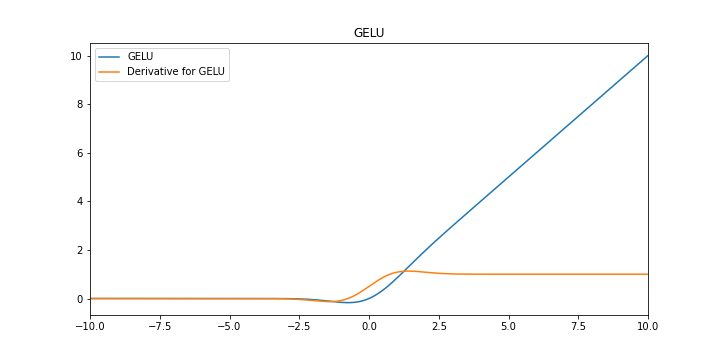
\includegraphics[width=\linewidth]{./imgs/GELU.png}


% Truely softmax = argmax


(d)
The four types of linear transformations are: rotations, zooming, flipping, and shearing.

The linear transformation can remap or change the input space or representation space, which help us get better representation and feature mapping.

For non linear transformation, we do not want a combined linear layer if all the layers are linear. For increasing the non-linearity and solve the non-linear tasks, we should use a non-linear layer. From one prespective, nonlinear transformation can map the task to a linear seperable task, just like we usually take linear layer as last layer. (before logit, for classification, and we do not consider the softmax as a layer)

(e)

When we increasing the batch size, the learning rate should be decreased.
When we decrease the batch size, the learning rate should be increased.

